\setlength{\columnsep}{3pt}
\begin{flushleft}
	\bigskip
	
	Things to note about array:
	\begin{itemize}
		\item In Java, every array is an Object.
		\item \textbf{"new"} operator is used to create an object.
		\item Hence, we can create array by using \textbf{new} operator.
	\end{itemize}
	
	
	\begin{itemize}
		
		\item \textbf{One dimensional array creation}:
		
		\begin{tcolorbox}[breakable,notitle,boxrule=1pt,colback=pink,colframe=pink]
			\color{black}
			\fontdimen2\font=8pt
			Syntax:  \newline
			int[] a = new int[4];
			\fontdimen2\font=4pt
		\end{tcolorbox}
		
		
		\begin{figure}[h!]
			\centering
			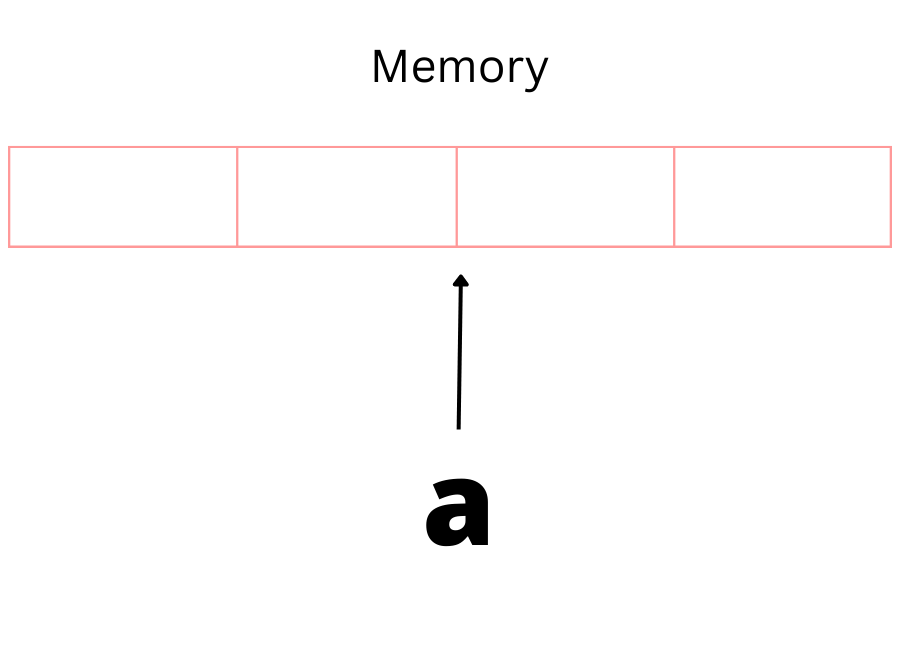
\includegraphics[scale=.45]{content/chapter4/images/array.png}
		\end{figure}	
		
		Important:
		\begin{itemize}
			\item At the time of array creation, \textbf{size should be mentioned compulsorily.}
			\item An array can be of zero size.
			\begin{tcolorbox}[breakable,notitle,boxrule=-0pt,colback=code,colframe=code]
				\color{black}
				\fontdimen2\font=8pt
				int[] x = new int[]; \xmark \par
				int[] x = new int[6]; \cmark  \par
				int[] x = new int[0]; \cmark 
				\fontdimen2\font=4pt
			\end{tcolorbox}
			
			\item Java compiler will never throw error for negative size of array. However, Java Virtual Machine will throw runtime error: \textbf{NegativeArraySizeException}.
			\begin{tcolorbox}[breakable,notitle,boxrule=-0pt,colback=code,colframe=code]
				\color{black}
				\fontdimen2\font=8pt
				int[] x = new int[-3]; \xmark
				\fontdimen2\font=4pt
			\end{tcolorbox}
			
			\item Allowed data types for mentioning array size are:
			\begin{itemize}
				\item integer
				\item byte
				\item short
				\item char
			\end{itemize}
			
			\begin{figure}[h!]
				\centering
				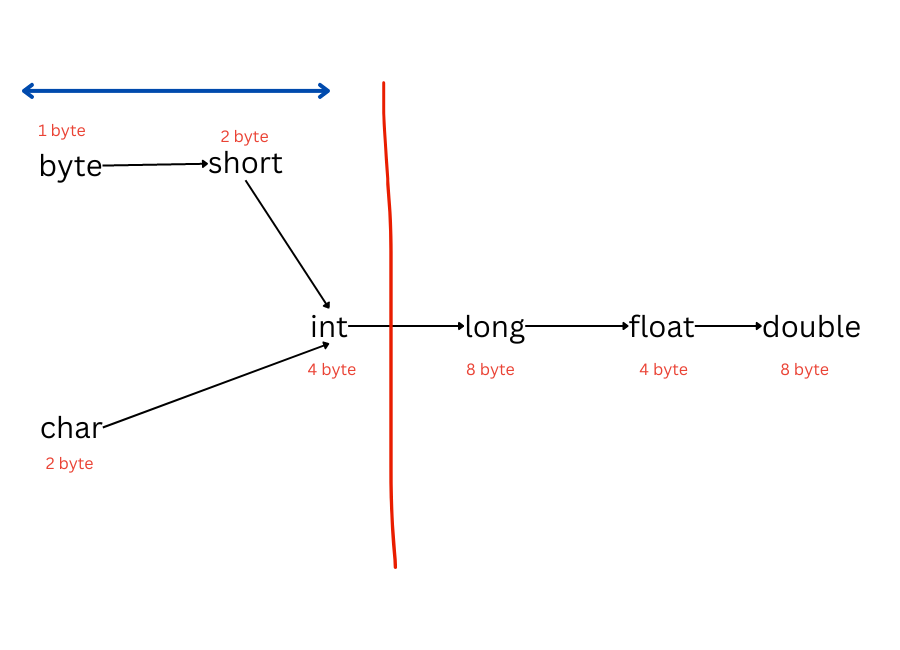
\includegraphics[scale=.45]{content/chapter4/images/allow.png}
			\end{figure}	
			
			\begin{tcolorbox}[breakable,notitle,boxrule=-0pt,colback=code,colframe=code]
				\color{black}
				\fontdimen2\font=8pt
				int[] x = new int[10]; \cmark \par
				int[] x = new int['a']; \cmark \par
				byte b = 20; \par
				int[] x = new int[b]; \cmark \par
				short s = 30; \par
				int[] x = new int[s]; \cmark \par
				\fontdimen2\font=4pt
			\end{tcolorbox}
			
			\newpage
			Below array creation will result in error:
			\begin{tcolorbox}[breakable,notitle,boxrule=-0pt,colback=code,colframe=code]
				\color{black}
				\fontdimen2\font=8pt
				int[] x = new int[10l]; \xmark \par
				int[] x = new int[3.5]; \xmark 
				\fontdimen2\font=4pt
			\end{tcolorbox}
			
			\item Maximum size of array can be 2147483647:
			\begin{tcolorbox}[breakable,notitle,boxrule=-0pt,colback=code,colframe=code]
				\color{black}
				\fontdimen2\font=8pt
				int[] x = new int[2147483647]; \cmark \par
				int[] x = new int[2147483648]; \xmark 
				\fontdimen2\font=4pt
			\end{tcolorbox}
			
			\item For every array type, corresponding classes are available and these classes are part of Java language and not available to the programmer level.
			\bigskip
			\bigskip
			\begin{tabulary}{1.0\textwidth}{|p{12em}|p{12em}|}
				\toprule
				\textbf{Array type} & \textbf{Corresponding class name} \\
				\midrule
				int[] & [I \\
				\hline
				int[][] & [[I \\
				\hline
				double[] & [D \\
				\hline
				short[] & [S \\
				\hline
				byte[] & [B \\
				\hline
				boolean[] & [Z \\
				\bottomrule
			\end{tabulary}
			\bigskip
			Eg: You can find name of class for different array type:
			\begin{tcolorbox}[breakable,notitle,boxrule=-0pt,colback=code,colframe=code]
				\color{black}
				\fontdimen2\font=8pt
				int[] a = new int[3]; \newline
				System.out.println(a.getClass().getName());
				\fontdimen2\font=4pt
			\end{tcolorbox}
			
			Output:
			\begin{tcolorbox}[breakable,notitle,boxrule=-0pt,colback=output,colframe=output]
				\color{black}
				\fontdimen2\font=8pt
				[I			
				\fontdimen2\font=4pt
			\end{tcolorbox}	
			
			
		\end{itemize}
		
		\newpage
		\item \textbf{Two-dimensional array creation}:
		\begin{itemize}
			\item In Java, two dimensional array is not implmeneted using matrix approach.
			\item Array of arrays approach is followed for multi-dimensional array creation.
			\item Advantage of array of arrays approach is improved memory utilisation.
			
			
		\end{itemize}
		\bigskip
		
		There are different ways of creating two-dimensional array.
		\begin{itemize}
			\item \textbf{Base size}: In this we specifiy the size of first dimension at the time of array creation.
			\begin{tcolorbox}[breakable,notitle,boxrule=-0pt,colback=code,colframe=code]
				\color{black}
				\fontdimen2\font=8pt
				int[][] x = new int[2][]; \par
				x[0] = new int[2]; \par
				x[1] = new int[3];
				\fontdimen2\font=4pt
			\end{tcolorbox}
			
			\begin{figure}[h!]
				\centering
				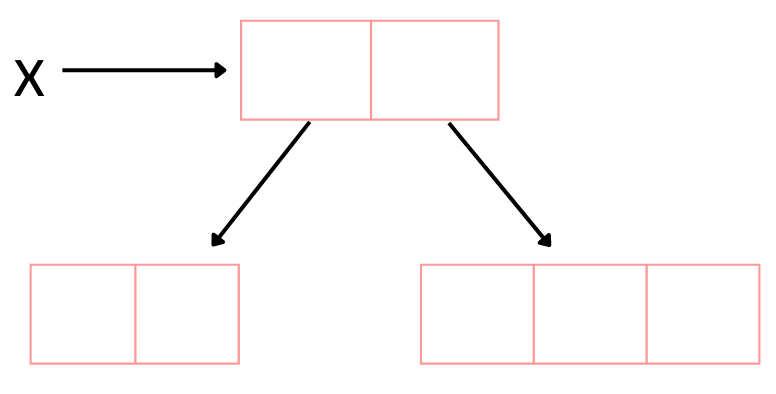
\includegraphics[scale=.45]{content/chapter4/images/two.png}
			\end{figure}	
			
			\newpage
			
		\end{itemize}
		
		\item Three-dimensional array creation:
		\begin{tcolorbox}[breakable,notitle,boxrule=-0pt,colback=code,colframe=code]
			\color{black}
			\fontdimen2\font=8pt
			int[][][] x = new int[2][][]; \par
			x[0] = new int[3][]; \par
			x[0][0] = new int[1]; \par
			x[0][1] = new int[2]; \par
			x[0][2] = new int[3]; \par
			x[1] = new int[2][2];
			\fontdimen2\font=4pt
		\end{tcolorbox}
		
		\begin{figure}[h!]
			\centering
			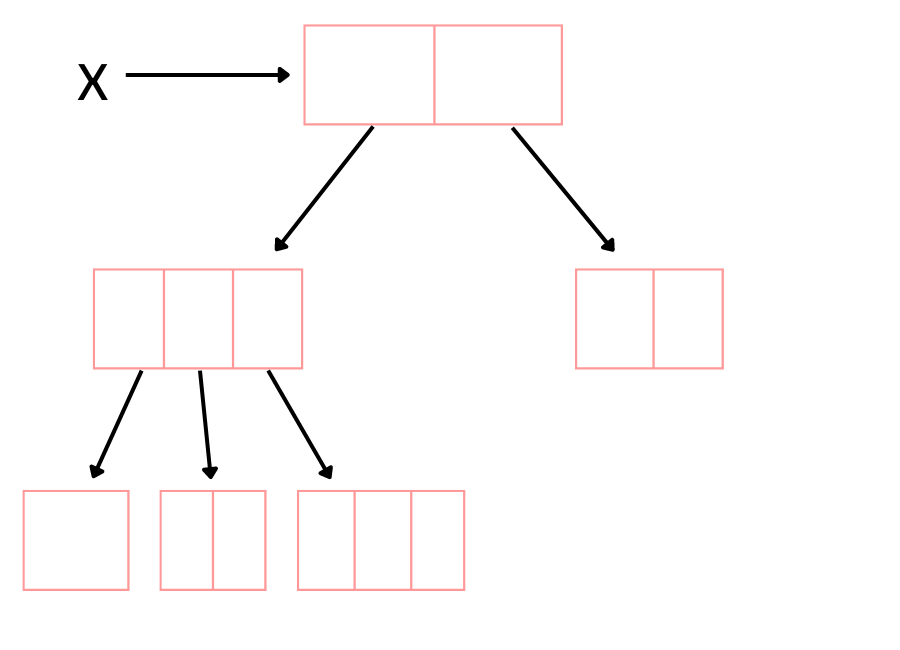
\includegraphics[scale=.45]{content/chapter4/images/three.png}
		\end{figure}
		
		
	\end{itemize}
	
	
	
\end{flushleft}

\newpage




